\begin{figure}[H]
    \centering
    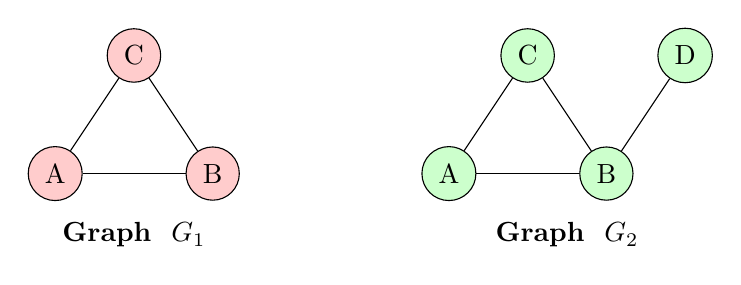
\begin{tikzpicture}
        \node[circle, draw, fill=red!20] (A1) at (0,0) {A};
        \node[circle, draw, fill=red!20] (B1) at (2,0) {B};
        \node[circle, draw, fill=red!20] (C1) at (1,1.5) {C};
        \draw (A1) -- (B1);
        \draw (A1) -- (C1);
        \draw (B1) -- (C1);
        \node[align=center, below] at (1, -0.5) {\textbf{Graph } $G_1$};
        \node[circle, draw, fill=green!20] (A2) at (5,0) {A};
        \node[circle, draw, fill=green!20] (B2) at (7,0) {B};
        \node[circle, draw, fill=green!20] (C2) at (6,1.5) {C};
        \node[circle, draw, fill=green!20] (D2) at (8,1.5) {D};
        \draw (A2) -- (B2);
        \draw (A2) -- (C2);
        \draw (B2) -- (C2);
        \draw (B2) -- (D2);
        \node[align=center, below] at (6.5, -0.5) {\textbf{Graph } $G_2$};
        
        
    \end{tikzpicture}
    \caption{Pair of graphs to demonstre Graph Edit Distance.}
    \label{fig:ged-graphs}
\end{figure}